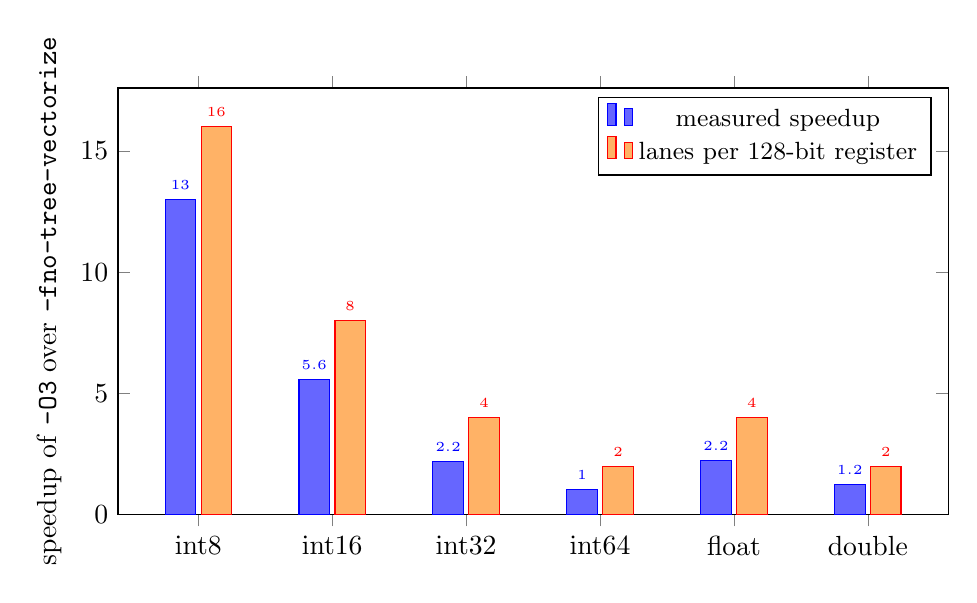
\begin{tikzpicture}
\begin{axis}[ybar, width=\textwidth, height=7cm, bar width=11pt, ymin=0, ylabel={speedup of \texttt{-O3} over \texttt{-fno-tree-vectorize}}, symbolic x coords={int8,int16,int32,int64,float,double}, xtick=data,
  legend style={font=\small, at={(0.98,0.98)}, anchor=north east}, enlarge x limits=0.12, nodes near coords, nodes near coords style={font=\tiny}, every node near coord/.append style={/pgf/number format/.cd, fixed, precision=1}]
\addplot+[fill=blue!60] coordinates {(int8,12.994) (int16,5.577) (int32,2.198) (int64,1.032) (float,2.225) (double,1.235)};
\addlegendentry{measured speedup}
\addplot+[fill=orange!60] coordinates {(int8,16) (int16,8) (int32,4) (int64,2) (float,4) (double,2)};
\addlegendentry{lanes per 128-bit register}
\end{axis}
\end{tikzpicture}